In this section, the numerical simulation is performed
for the curved channel with stent as in the section 
\ref{canal curvado com stent}, however the quadratic element
was used. The domain was discretized using 18689 nodes and 
9070 quadratic triangular elements. 

\medskip 
The \ref{quad velocity evolution curved stent} shows the unsteady state 
velocity profile in the middle section channel, that is, 
$x=5.0R$. 
As expected, the numerical solution converges to a similar profile to
the Half Poiseuille, as presented in the section \ref{half poiseuille sec}. However, it is possible to observe an inversion of the velocity
field sense at the top of the figure.
This inversion occurs in the region that is
located between the stents strut semi-circles.
It is also possible to observe that the maximum horizontal velocity field 
in curvel channel reaches the $u=3.25$ non-dimensional value, that is, 
more than 3 times the blood velocity in coronary artery
without atherosclerosis and stent strut placed. 
This increase can influence the dynamics of blood flow
and its biological processes and a more detailed analysis
should be performed.

\vspace{1cm}
\begin{figure}[H]
     \caption{
The unsteady state velocity profile in the middle ($x=5.0R$) of the quadratic curved channel with drug-eluting stent.}
     \centering
     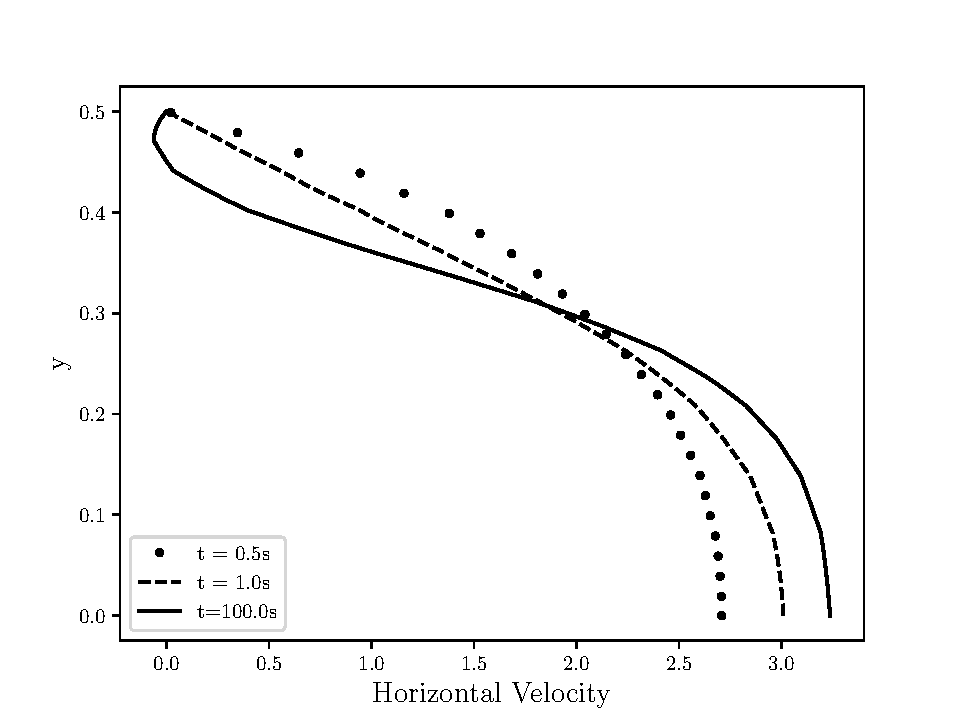
\includegraphics[scale=1]{./02_chaps/cap_solution/figure/vel_quadCurvedStrut_evol.pdf}\\
     \label{quad velocity evolution curved stent}
\end{figure}

\newpage
The \ref{velocity field curved stent} presents the evolution in 
time and space of the velocity field for half of the domain
due to the symmetry of the solution. 
The velocity field is represented with non-dimensional values 
where the red color refers to the $u=3.25$ value and the blue color 
$u=0$ value. Conveting to dimensional values, 
we have $u=39.0cm/s$ and $u=0cm/s$ respectively.
As can be seen, the region with the lowest horizontal velocity 
magnitude is found close to the boundary where the no-slip
condition is applied. Whereas, it is increase close to 
the symmetric axis. Moreover, the largest horizontal velocity value
is found in the maximum contraction region.


\vspace{1cm} 
\begin{figure}[H]
     \caption{
Temporal and spatial evolution of the velocity field for quadratric curved channel with
drug-eluting stent.}
     \begin{minipage}{.50\linewidth}
      \centering
      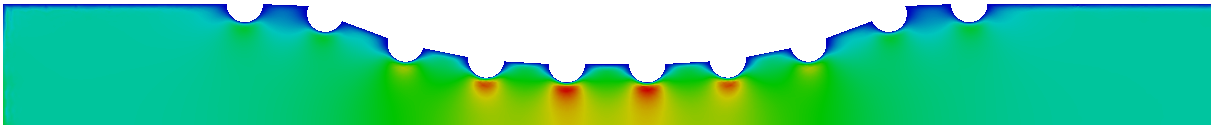
\includegraphics[scale=0.18]{./02_chaps/cap_solution/figure/vel_quadCurvedStrut1.png}\\
      t = 0.1s
     \end{minipage}%
     \begin{minipage}{.50\linewidth}
      \centering
      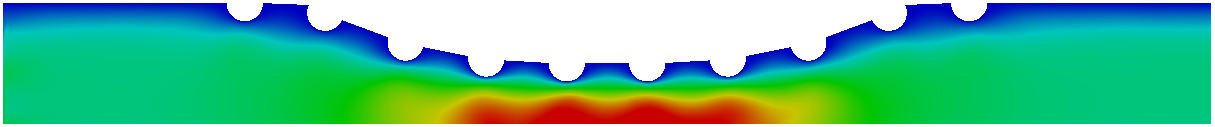
\includegraphics[scale=0.18]{./02_chaps/cap_solution/figure/vel_quadCurvedStrut2.png}\\
      t = 0.5s
     \end{minipage}
     \begin{minipage}{.50\linewidth}
     \medskip
      \centering
      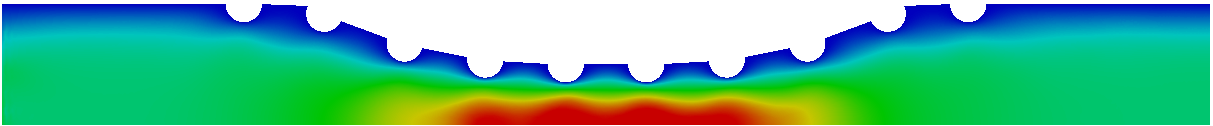
\includegraphics[scale=0.18]{./02_chaps/cap_solution/figure/vel_quadCurvedStrut3.png}\\
      t = 1.0s
     \end{minipage}%
     \begin{minipage}{.50\linewidth}
     \medskip
      \centering
      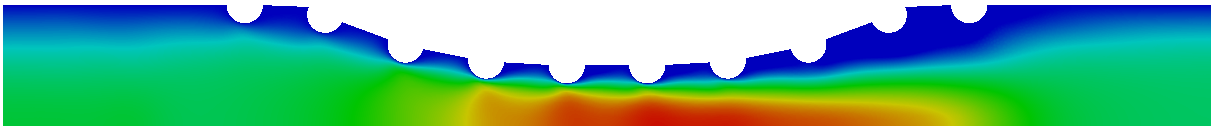
\includegraphics[scale=0.18]{./02_chaps/cap_solution/figure/vel_quadCurvedStrut4.png}\\
      t = 3.0s
     \end{minipage}
     \begin{minipage}{.50\linewidth}
      \centering
      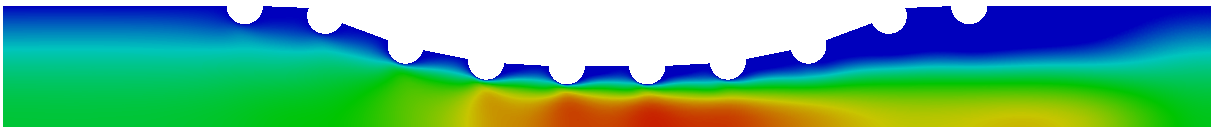
\includegraphics[scale=0.18]{./02_chaps/cap_solution/figure/vel_quadCurvedStrut5.png}\\
      t = 5.0s
     \end{minipage}%
     \begin{minipage}{.50\linewidth}
      \centering
      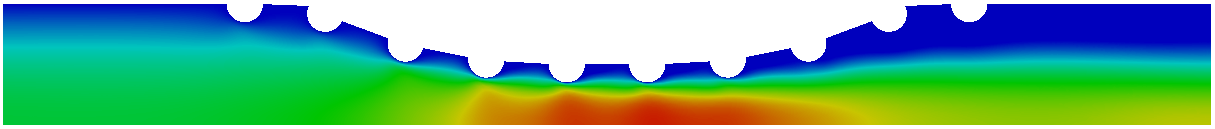
\includegraphics[scale=0.18]{./02_chaps/cap_solution/figure/vel_quadCurvedStrut6.png}\\
      t = 7.0s
     \end{minipage}
     \begin{minipage}{.50\linewidth}
     \medskip
      \centering
      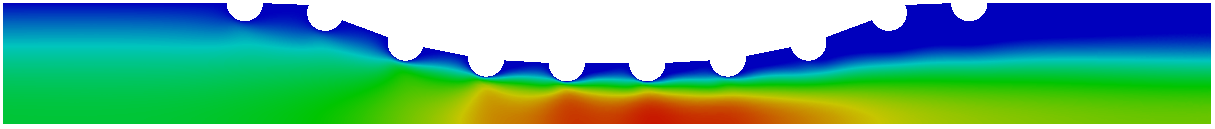
\includegraphics[scale=0.18]{./02_chaps/cap_solution/figure/vel_quadCurvedStrut7.png}\\
      t = 10.0s
     \end{minipage}%
     \begin{minipage}{.50\linewidth}
     \medskip
      \centering
      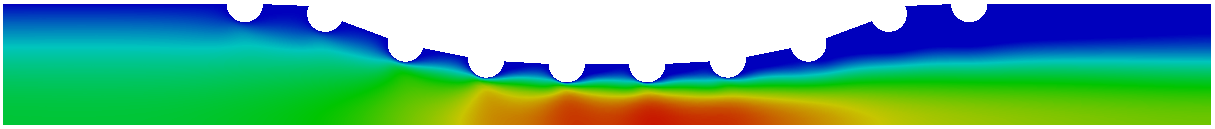
\includegraphics[scale=0.18]{./02_chaps/cap_solution/figure/vel_quadCurvedStrut8.png}\\
      t = 100.0s
     \end{minipage}\\[10pt]
      \centering
      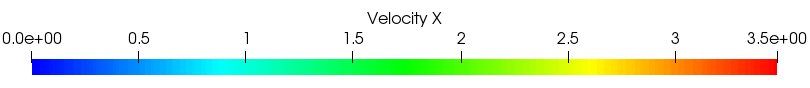
\includegraphics[scale=0.5]{./02_chaps/cap_solution/figure/vel_CurvedStrutScale.png}\\
     \medskip
     \label{quad velocity field curved stent}
\end{figure}


\vspace{1cm}
The \ref{quad conc field curved stent sc 1} and
\ref{quad conc field curved stent sc 10} show the 
temporal and spatial evolution 
of the concentration field for several \textit{Schmidt} number, 
such as: $1$ and $10$ respectively for quadratic triangular element. 
The concentration field is 
represented with the non-dimensional values where the red color 
represents $100$\% and the blue color represents $0$\% 
of the diffused concentration in the bloodstream. 

\bigskip
It is possible to observe in the \ref{quad conc field curved stent sc 1}
that the concentration field is significally more diffuse than in the
\ref{quad conc field curved stent sc 10}, where the Schmidt number
is 10 times higher. This means that a large portion of the
diffused drug in bloodstream is quickly spread in the
$Sc=1$ case.
Moreover, in both cases, the concentration field
is more dispersed at the end of the curved channel due to
the sense of the blood flow. 

\bigskip

In comparison with the linear element in the section 
\ref{canal curvado com stent}, it is possible 
to observe at the end of the channel that the quadratic 
element has less diffusion of the concentration field. 
This effect may be due to an improvement in the accuracy 
of the simulation, but more detailed analyzes are necessary.


\vspace{1cm}
\begin{figure}[H]
     \caption{
Temporal and spatial evolution of the concentration fiel for quadratic curved channel with drug-eluting stent and $Sc=1$.}
     \begin{minipage}{.50\linewidth}
      \centering
      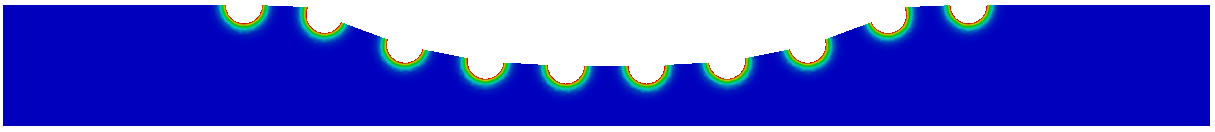
\includegraphics[scale=0.18]{./02_chaps/cap_solution/figure/conc1_quadCurvedStrut1.png}\\
      t = 0.1s
     \end{minipage}%
     \begin{minipage}{.50\linewidth}
      \centering
      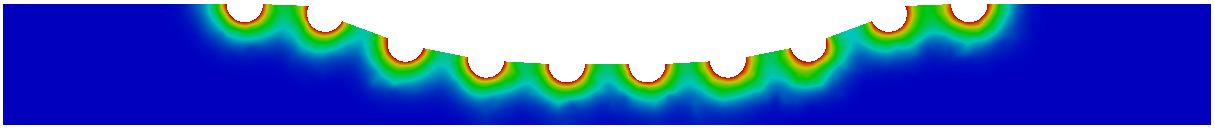
\includegraphics[scale=0.18]{./02_chaps/cap_solution/figure/conc1_quadCurvedStrut2.png}\\
      t = 0.5s
     \end{minipage}
     \begin{minipage}{.50\linewidth}
     \medskip
      \centering
      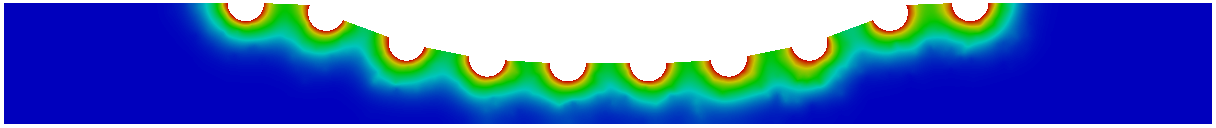
\includegraphics[scale=0.18]{./02_chaps/cap_solution/figure/conc1_quadCurvedStrut3.png}\\
      t = 1.0s
     \end{minipage}%
     \begin{minipage}{.50\linewidth}
     \medskip
      \centering
      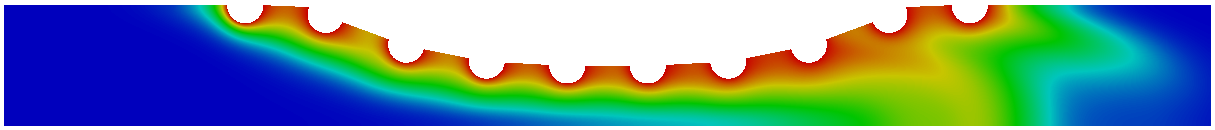
\includegraphics[scale=0.18]{./02_chaps/cap_solution/figure/conc1_quadCurvedStrut4.png}\\
      t = 3.0s
     \end{minipage}
     \begin{minipage}{.50\linewidth}
      \centering
      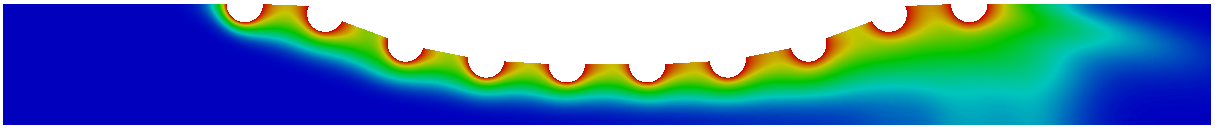
\includegraphics[scale=0.18]{./02_chaps/cap_solution/figure/conc1_quadCurvedStrut5.png}\\
      t = 5.0s
     \end{minipage}%
     \begin{minipage}{.50\linewidth}
      \centering
      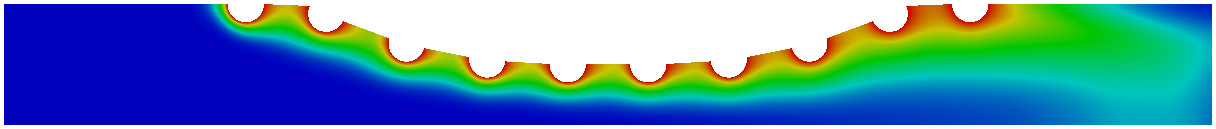
\includegraphics[scale=0.18]{./02_chaps/cap_solution/figure/conc1_quadCurvedStrut6.png}\\
      t = 7.0s
     \end{minipage}
     \begin{minipage}{.50\linewidth}
     \medskip
      \centering
      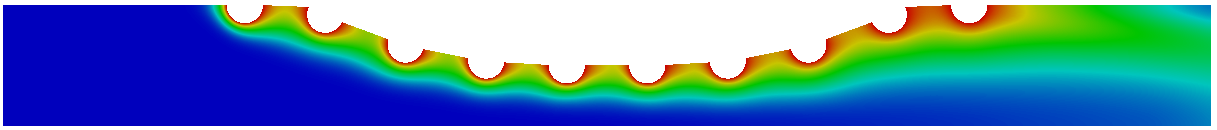
\includegraphics[scale=0.18]{./02_chaps/cap_solution/figure/conc1_quadCurvedStrut7.png}\\
      t = 10.0s
     \end{minipage}%
     \begin{minipage}{.50\linewidth}
     \medskip
      \centering
      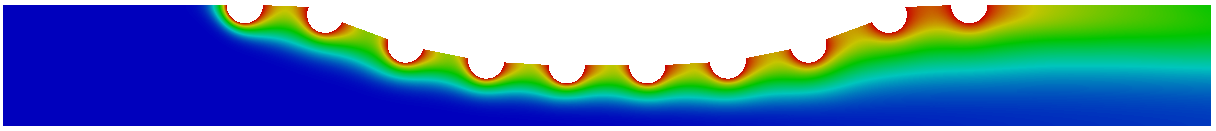
\includegraphics[scale=0.18]{./02_chaps/cap_solution/figure/conc1_quadCurvedStrut8.png}\\
      t = 100.0s
     \end{minipage}\\[10pt]
      \centering
      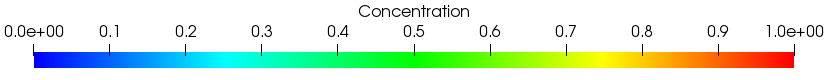
\includegraphics[scale=0.5]{./02_chaps/cap_solution/figure/conc1_CurvedStrutScale.png}\\
     \medskip
     \label{quad conc field curved stent sc 1}
\end{figure}



\begin{figure}[H]
    \caption{
Temporal and spatial evolution of the concentration fiel for quad curved channel with drug-eluting stent and $Sc=10$.}
     \begin{minipage}{.50\linewidth}
      \centering
      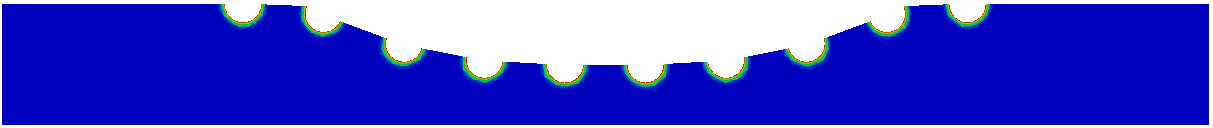
\includegraphics[scale=0.18]{./02_chaps/cap_solution/figure/conc10_quadCurvedStrut1.png}\\
      t = 0.1s
     \end{minipage}%
     \begin{minipage}{.50\linewidth}
      \centering
      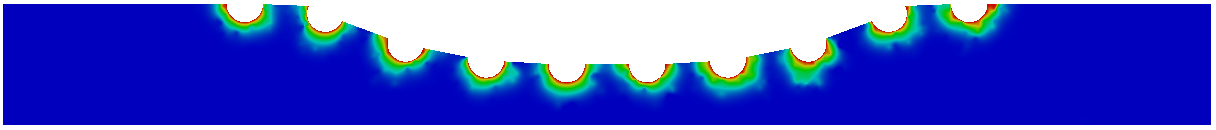
\includegraphics[scale=0.18]{./02_chaps/cap_solution/figure/conc10_quadCurvedStrut2.png}\\
      t = 0.5s
     \end{minipage}
     \begin{minipage}{.50\linewidth}
     \medskip
      \centering
      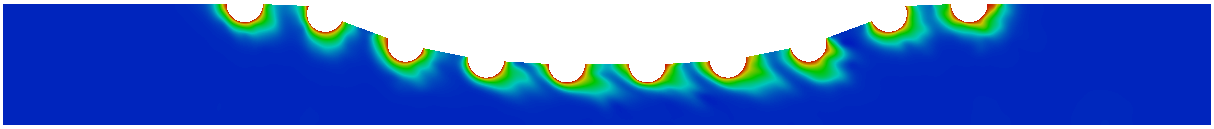
\includegraphics[scale=0.18]{./02_chaps/cap_solution/figure/conc10_quadCurvedStrut3.png}\\
      t = 1.0s
     \end{minipage}%
     \begin{minipage}{.50\linewidth}
     \medskip
      \centering
      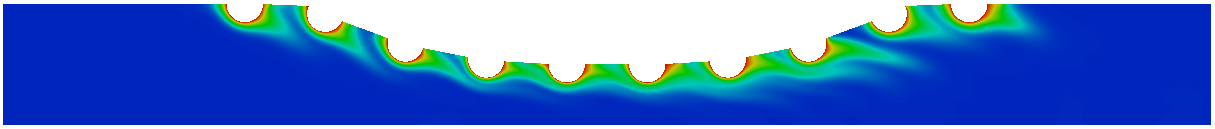
\includegraphics[scale=0.18]{./02_chaps/cap_solution/figure/conc10_quadCurvedStrut4.png}\\
      t = 3.0s
     \end{minipage}
     \begin{minipage}{.50\linewidth}
      \centering
      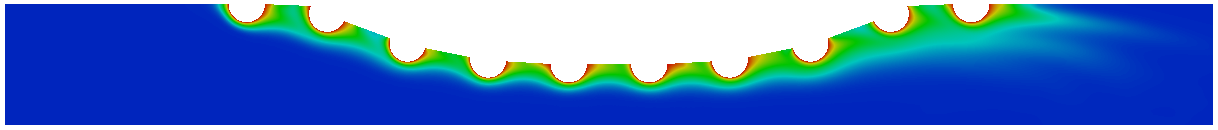
\includegraphics[scale=0.18]{./02_chaps/cap_solution/figure/conc10_quadCurvedStrut5.png}\\
      t = 5.0s
     \end{minipage}%
     \begin{minipage}{.50\linewidth}
      \centering
      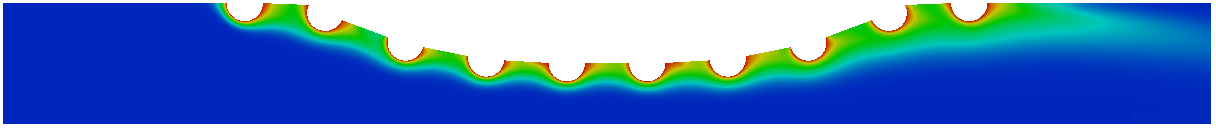
\includegraphics[scale=0.18]{./02_chaps/cap_solution/figure/conc10_quadCurvedStrut6.png}\\
      t = 7.0s
     \end{minipage}
     \begin{minipage}{.50\linewidth}
     \medskip
      \centering
      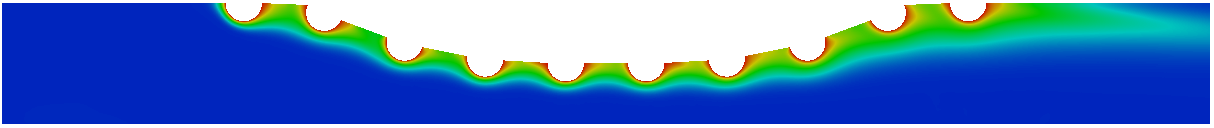
\includegraphics[scale=0.18]{./02_chaps/cap_solution/figure/conc10_quadCurvedStrut7.png}\\
      t = 10.0s
     \end{minipage}%
     \begin{minipage}{.50\linewidth}
     \medskip
      \centering
      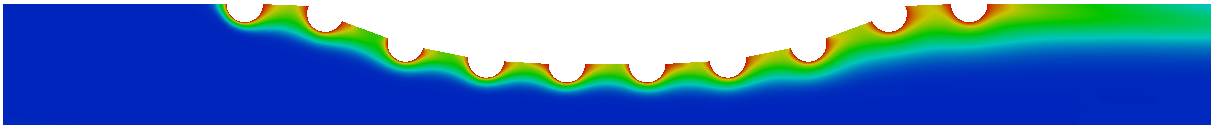
\includegraphics[scale=0.18]{./02_chaps/cap_solution/figure/conc10_quadCurvedStrut8.png}\\
      t = 100.0s
     \end{minipage}\\[10pt]
      \centering
      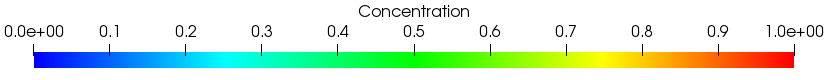
\includegraphics[scale=0.5]{./02_chaps/cap_solution/figure/conc1_CurvedStrutScale.png}\\
     \medskip
     \label{quad conc field curved stent sc 10}
\end{figure}


